\documentclass{beamer}
\usepackage{tikz}
\usepackage[all]{xy}
\usepackage{amsmath,amssymb}
\usepackage{hyperref}
\usepackage{graphicx}
\usepackage{algorithmic}
\usepackage{multirow}

\DeclareMathOperator*{\argmin}{arg\,min}
\DeclareMathOperator*{\Lik}{Lik}
\DeclareMathOperator*{\PoissonLoss}{PoissonLoss}
\DeclareMathOperator*{\Peaks}{Peaks}
\DeclareMathOperator*{\Segments}{Segments}
\DeclareMathOperator*{\argmax}{arg\,max}
\DeclareMathOperator*{\maximize}{maximize}
\DeclareMathOperator*{\minimize}{minimize}
\newcommand{\sign}{\operatorname{sign}}
\newcommand{\RR}{\mathbb R}
\newcommand{\ZZ}{\mathbb Z}
\newcommand{\NN}{\mathbb N}
\newcommand{\z}{$z = 2, 4, 3, 5, 1$} 

\newcommand{\algo}[1]{\textcolor{#1}{#1}}
\definecolor{PDPA}{HTML}{66C2A5}
\definecolor{CDPA}{HTML}{FC8D62}
\definecolor{GPDPA}{HTML}{4D4D4D}

% Set transparency of non-highlighted sections in the table of
% contents slide.
\setbeamertemplate{section in toc shaded}[default][100]
\AtBeginSection[]
{
  \setbeamercolor{section in toc}{fg=red} 
  \setbeamercolor{section in toc shaded}{fg=black} 
  \begin{frame}
    \tableofcontents[currentsection]
  \end{frame}
}

\begin{document}

\title{Introduction to machine learning and neural networks}

\author{
  Toby Dylan Hocking\\
  toby.hocking@nau.edu\\
  toby.hocking@r-project.org\\
}

\maketitle


\section{Fully connected multi-layer Neural Networks}

\begin{frame}
  \frametitle{Supervised learning setup}
  \begin{itemize}
  \item Have an input $\mathbf x\in\mathbb R^d$ -- a vector of $d$
    real numbers.
  \item And an output $y$ (real number: regression, integer ID:
    classification).
  \item Want to learn a prediction function $f(\mathbf x) = y$ that
    will work on a new input.
  \item In a neural network with $L-1$ hidden layers the function $f$
    is defined using composition of $L$ functions,
    $f(x)=f^{(L)}[\cdots f^{(1)}[x] ]\in\mathbb R$.
  \end{itemize}
\end{frame}

\begin{frame}
  \frametitle{Each function is matrix multiplication and activation}
  \begin{itemize}
  \item Prediction function $f(x)=f^{(L)}[\cdots f^{(1)}[x] ]\in\mathbb R$.
  \item Each function $l\in\{1,\dots, L\}$ is a matrix multiplication
    followed by an activation function:
    $f^{(l)}[z] = \sigma^{(l)}[ W^{(l)} z ]$ where
    $W^{(l)}\in\mathbb R^{u^{(l)}\times u^{(l-1)}}$ is a weight matrix
    to learn, and $z\in\mathbb R^{u^{(l-1)}}$ is the input vector to
    that layer.
\item In regression the last activation function must return
a real number prediction so it is fixed to the identity:
$\sigma^{(L)}[z]=z$.
\item The other activation functions must be
non-linear, e.g. 
logistic/sigmoid $\sigma(z)=1/(1+\exp(-z))$ or rectified linear units (ReLU) 
$$
\sigma(z)=
\begin{cases}
  z & \text{ if } z>0,\\
  0 & \text{ else.}
\end{cases}
$$ 
\end{itemize}
\end{frame}

\begin{frame}
  \frametitle{Non-linear activation functions}
$
\sigma(z)=
\begin{cases}
  z & \text{ if } z>0,\\
  0 & \text{ else.}
\end{cases}
$
  \hskip 1in
  $\sigma(z)=1/(1+\exp(-z))$

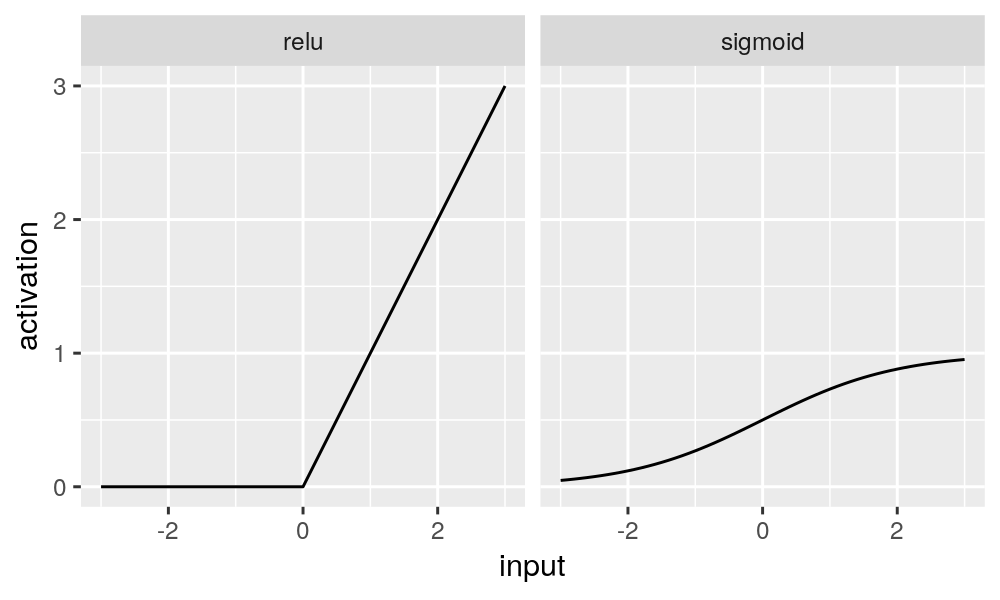
\includegraphics[width=\textwidth]{figure-activations}
\end{frame}

\begin{frame}
  \frametitle{Network size}
For binary classification
with inputs $x\in\mathbb R^d$, the overall neural network architecture
is $(u^{(0)}=d, u^{(1)}, \dots, u^{(L-1)}, u^{(L)}=1)$, where
$u^{(1)},\dots, u^{(L-1)}\in\mathbb Z_+$ are positive integers
(hyper-parameters that control the number of units in each hidden
layer, and the size of the parameter matrices $W^{(l)}$).
\begin{itemize}
\item First layer size $u^{(0)}$ is fixed to input size.
\item Last layer size $u^{(L)}$ is fixed to output size.
\item Number of layers and hidden layer sizes
  $u^{(1)},\dots, u^{(L-1)}$ must be chosen (by you).
\end{itemize}
\end{frame}

\begin{frame}
  \frametitle{Network diagrams}
Neural network diagrams show how each hidden unit (node) is computed by
applying the weights (edges) to the values of the hidden units at the previous
layer.

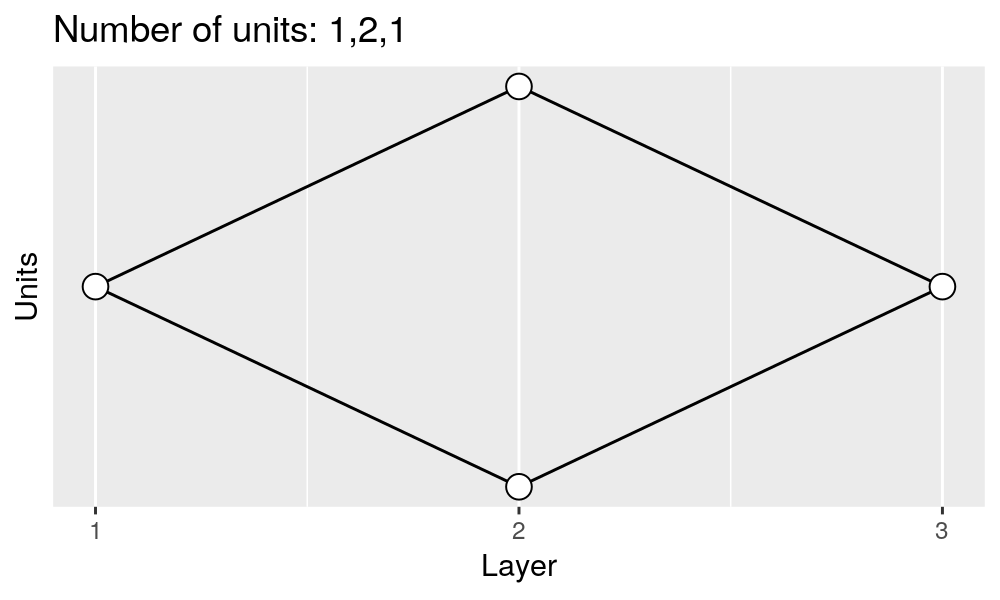
\includegraphics[width=\textwidth]{figure-architecture-reg2}
\end{frame}

\begin{frame}[fragile]
  \frametitle{torch code}
\begin{verbatim}
import torch
class Net(torch.nn.Module):
    def __init__(self):
        super(Net, self).__init__()
        n_hidden = 2
        self.act = torch.nn.Sigmoid()
        self.hidden = torch.nn.Linear(1, n_hidden)
        self.out = torch.nn.Linear(n_hidden, 1)
    def forward(self, x):
        x = self.act(self.hidden(x))
        x = self.out(x)
        return x
\end{verbatim}
\end{frame}

\begin{frame}
  \frametitle{Network diagrams}

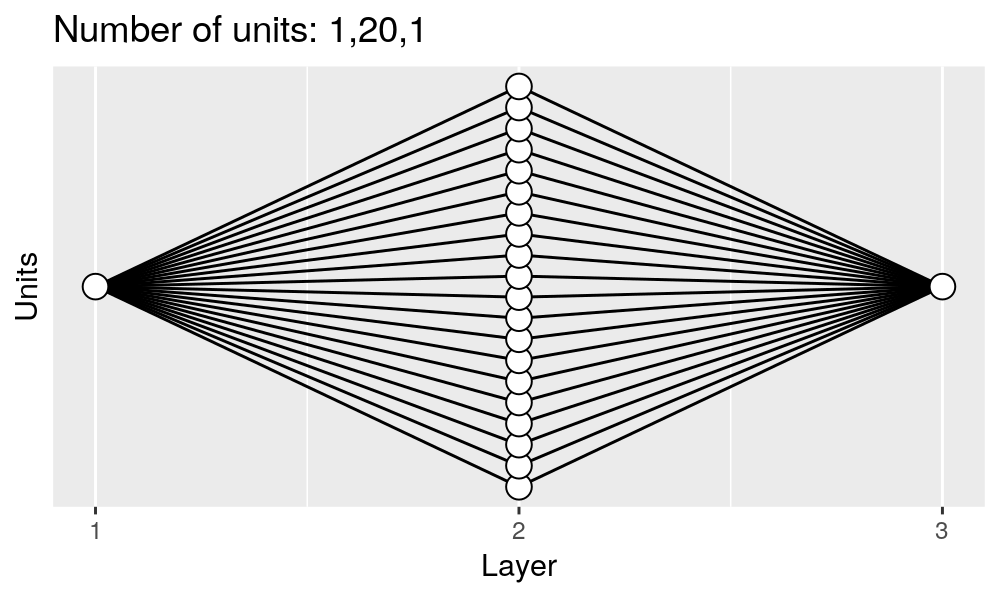
\includegraphics[width=\textwidth]{figure-architecture-reg20}
\end{frame}

\begin{frame}
  \frametitle{Network diagrams}

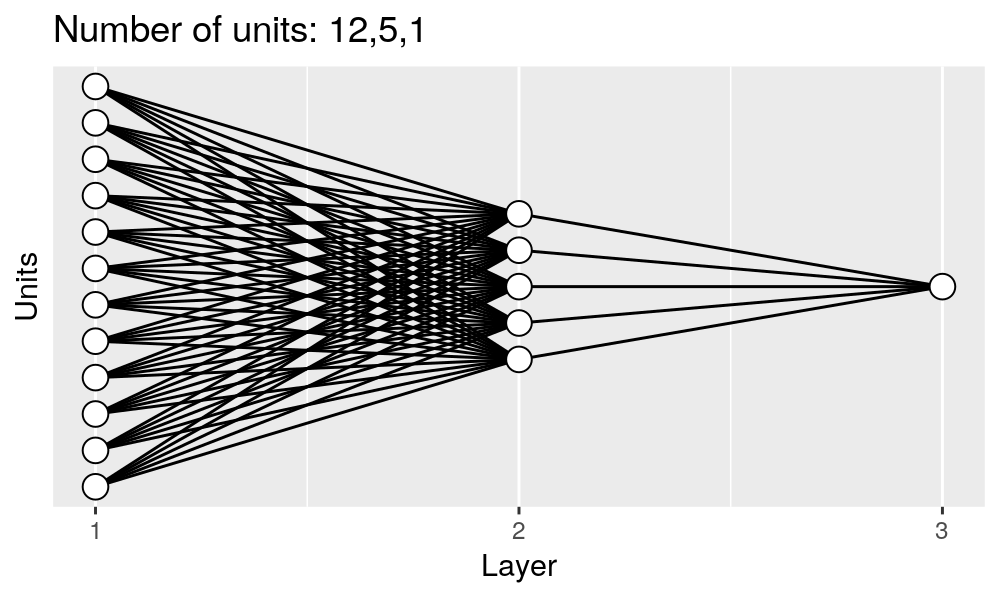
\includegraphics[width=\textwidth]{figure-architecture-oneOut}
\end{frame}

\begin{frame}[fragile]
  \frametitle{torch code}
\begin{verbatim}
import torch
class Net(torch.nn.Module):
    def __init__(self):
        super(Net, self).__init__()
        n_hidden = 5
        self.act = torch.nn.Sigmoid()
        self.hidden = torch.nn.Linear(12, n_hidden)
        self.out = torch.nn.Linear(n_hidden, 1)
    def forward(self, x):
        x = self.act(self.hidden(x))
        x = self.out(x)
        return x
\end{verbatim}
\end{frame}

\begin{frame}
  \frametitle{Network diagrams}

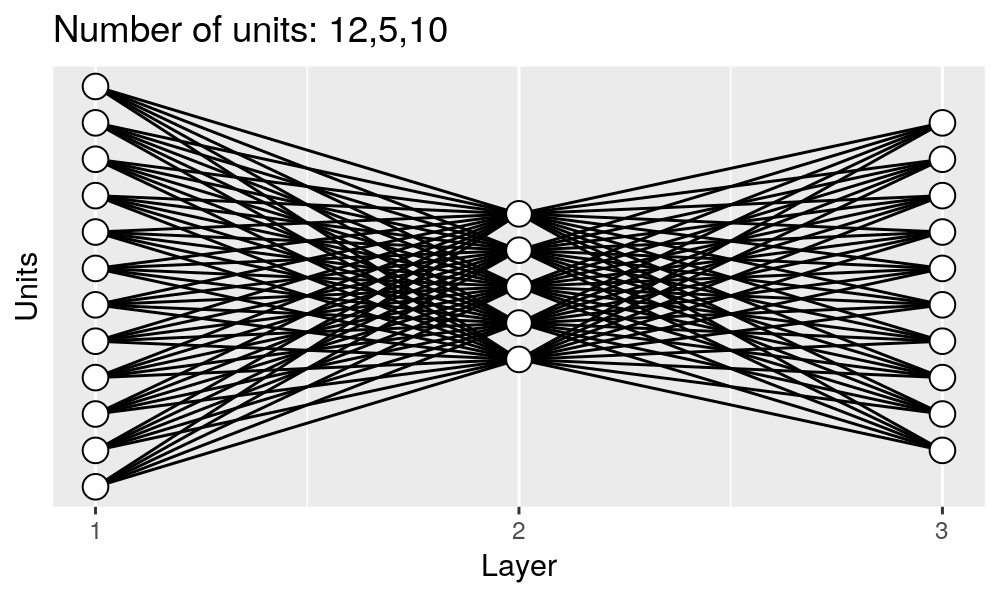
\includegraphics[width=\textwidth]{figure-architecture-tenOut}
\end{frame}

\begin{frame}
  \frametitle{Network diagrams}

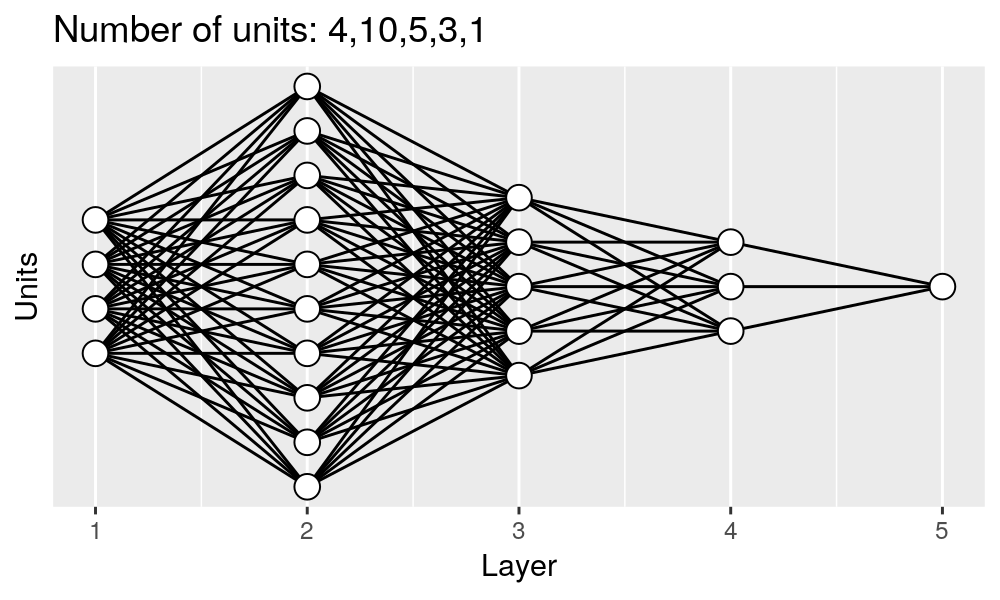
\includegraphics[width=\textwidth]{figure-architecture-fiveLayers}
\end{frame}

\begin{frame}
  \frametitle{Units in each layer}
We can write the units at each layer as
$h^{(0)},h^{(1)},\dots, h^{(L-1)}, h^{(L)}$ where
\begin{itemize}
\item $h^{(0)}=x\in\mathbb R^d$ is an input feature vector,
\item and
$h^{(L)}\in\mathbb R$ is the predicted output.
\end{itemize}
For
each layer $l\in \{1, \dots, L\}$ we have:
\begin{equation*}
  \label{eq:h_l}
  h_l = f^{(l)}\left[h^{(l-1)}\right] =
  \sigma^{(l)}\left[ W^{(l)} h^{(l-1)} \right].
\end{equation*}
Total number of parameters to learn is
$\sum_{l=1}^L u^{(l)} u^{(l-1)}.$

Quiz: how many parameters in a
neural network for $d=10$ inputs/features with one hidden layer with
$u=100$ units? (one output unit, ten output units)
\end{frame}

\section{Computing gradients and learning weights}

\begin{frame}
  \frametitle{Gradient descent learning}
  Basic idea of gradient descent learning algorithm is to iteratively
  update weights $\mathbf W = [W^{(1)}, \dots, W^{(L)} ]$ to improve
  predictions on the subtrain set.
  \begin{itemize}
  \item Need to define a loss function
    $\mathcal L(\mathbf W)$ which is differentiable, and
    takes small values for good predictions.
  \item Typically for regression we use the mean squared error, and
    for binary classification we use the logistic (cross entropy)
    loss.
  \item The gradient $\nabla \mathcal L(\mathbf W)$ is a
    function which tells us the local direction where the loss is most
    increasing.
  \end{itemize}
\end{frame}

\begin{frame}
  \frametitle{Loss functions}
  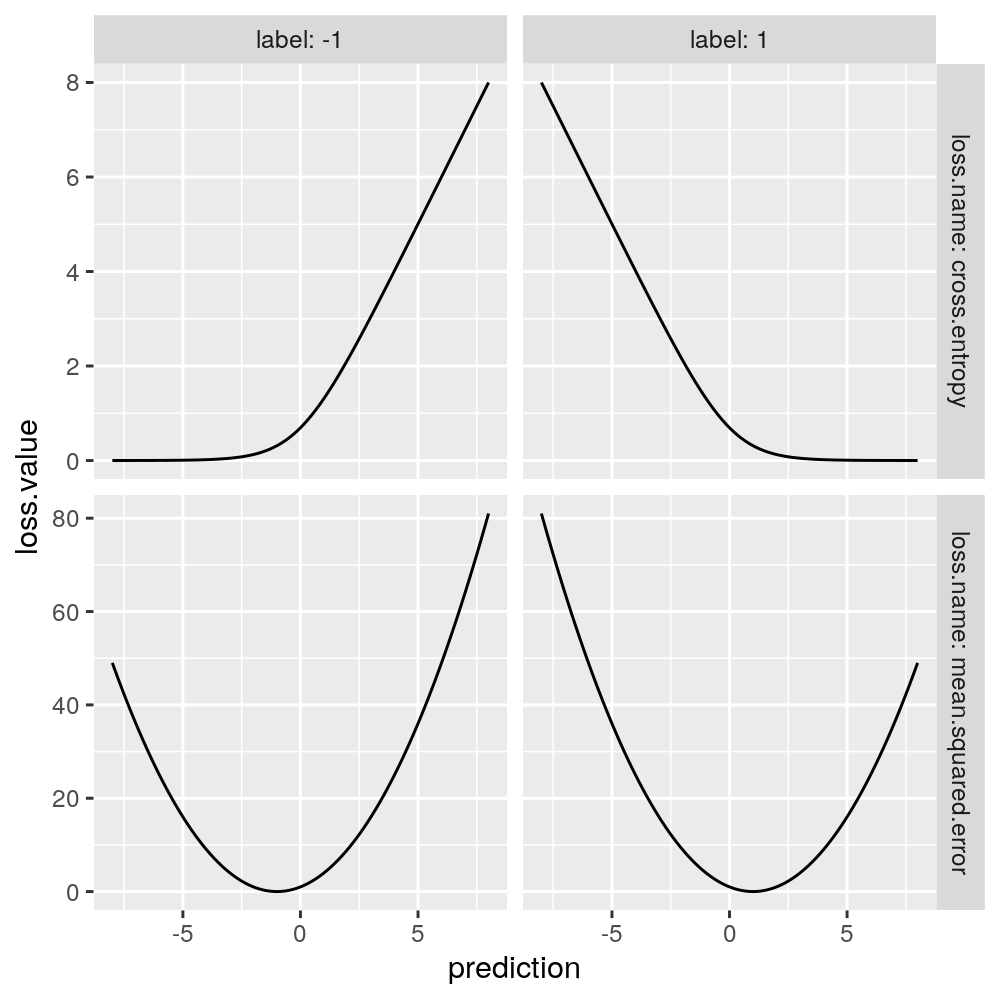
\includegraphics[width=0.8\textwidth]{figure-loss} 
\end{frame}

\begin{frame}
  \frametitle{Gradient descent animations}
  \url{https://yihui.org/animation/example/grad-desc/}

  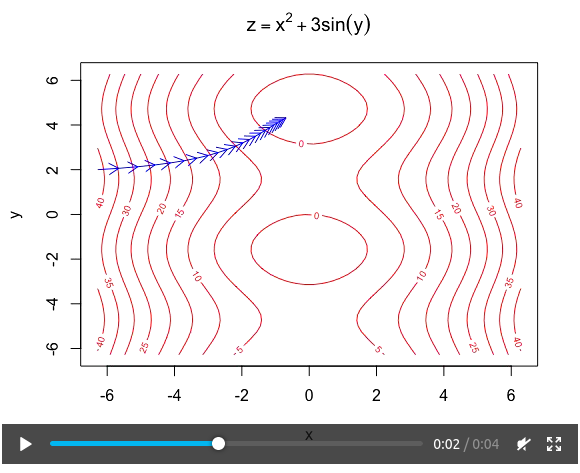
\includegraphics[width=0.9\textwidth]{screenshot-gradient-descent}
\end{frame}

\begin{frame}[fragile]
  \frametitle{Basic full gradient descent algorithm}
  \begin{itemize}
  \item Initialize weights $\mathbf W_0$ at some random values near
    zero (more complicated initializations possible).
  \item Since we want to decrease the loss, we take a step $\alpha$ in the
    opposite direction of the gradient,
  $$
\mathbf W_t = \mathbf W_{t-1} - \alpha \nabla \mathcal L(\mathbf W_{t-1})
$$
\item This is the \textbf{full} gradient method: batch size = $n$ =
  subtrain set size, so 1 step per epoch/iteration.
\end{itemize}

\begin{verbatim}
optimizer = torch.optim.SGD(net.parameters(), lr=0.03)
optimizer.zero_grad()
predictions = net(subtrain_inputs)
subtrain_loss = criterion(predictions, subtrain_outputs)
subtrain_loss.backward()
optimizer.step()
\end{verbatim}
\end{frame}

\begin{frame}[fragile]
  \frametitle{Stochastic gradient descent algorithm}
  \begin{itemize}
  \item Initialize weights $\mathbf W$ at some random values near
    zero (more complicated initializations possible).
  \item for each epoch $t$ from 1 to max epochs:
  \item for each batch $i$ from 1 to $n$:
  \item Let $\mathcal L( \mathbf W, \mathbf X_i, \mathbf y_i )$ be the loss with
    respect to the single observation in batch $i$.
$$
\mathbf W \gets \mathbf W - \alpha \nabla \mathcal L(\mathbf W, \mathbf X_i, \mathbf y_i)
$$
\item This is the \textbf{stochastic} gradient method: batch size = 1,
  so there are $n$ steps per epoch.
\end{itemize}

\begin{verbatim}
optimizer = torch.optim.SGD(net.parameters(), lr=0.03)
optimizer.zero_grad()
prediction = net(one_input)
one_loss = criterion(prediction, one_output)
one_loss.backward()
optimizer.step()
\end{verbatim}

\end{frame}

\begin{frame}[fragile]
  \frametitle{Batch (stochastic) gradient descent algorithm}
  \begin{itemize}
  \item Input: batch size $b$.
  \item Initialize weights $\mathbf W$ at some random values near
    zero (more complicated initializations possible).
  \item for each epoch $t$ from 1 to max epochs:
  \item for each batch $i$ from 1 to $\lceil n/b \rceil$:
  \item Let $\mathcal L( \mathbf W, \mathbf X_i, \mathbf y_i )$ be the loss with
    respect to the $b$ observations in batch $i$.
  $$
\mathbf W \gets \mathbf W - \alpha \nabla \mathcal L(\mathbf W, \mathbf X_i, \mathbf y_i)
$$
\item This is the \textbf{(mini)batch} stochastic gradient method:
  batch size = $b$, so there are $\lceil n/b \rceil$ steps per epoch.
\end{itemize}

\begin{verbatim}
optimizer = torch.optim.SGD(net.parameters(), lr=0.03)
optimizer.zero_grad()
prediction = net(batch_inputs)
batch_loss = criterion(prediction, batch_outputs)
batch_loss.backward()
optimizer.step()
\end{verbatim}

\end{frame}

\begin{frame}[fragile]
  \frametitle{Forward propagation}
Forward propagation is the computation of hidden units
$h^{(1)},\dots,h^{(L)}$ given the inputs $x$ and current parameters
$W^{(1)},\dots,W^{(L)}$.
\begin{verbatim}
    def forward(self, x):
        x = self.act(self.hidden(x))
        x = self.out(x)
        return x
\end{verbatim}
(start from input, apply weights and activation in each layer until
predicted output is computed)
\end{frame}

\begin{frame}[fragile]
  \frametitle{Back propagation}
Back propagation is the computation of gradients given current
parameters and hidden units.
\begin{itemize}
\item Start from loss function, compute gradient, send it to last
  layer, use chain rule, send gradient to previous layer, finally end
  up at first layer.
\item Result is gradients with respect to all weights in all layers.
\item Modern frameworks like torch do this using automatic
  differentiation based on your definition of the forward method and
  the loss function.
\end{itemize}

\begin{verbatim}
net = Net()
criterion = torch.nn.MSELoss()
optimizer = torch.optim.LBFGS(net.parameters(), lr=0.03)
optimizer.zero_grad()
pred = net(input_X_features)
loss = criterion(pred, output_y_labels)
loss.backward()
\end{verbatim}

\end{frame}

\begin{frame}
  \frametitle{Computation graph}
  % from cs499-spring2020/notes.tex
  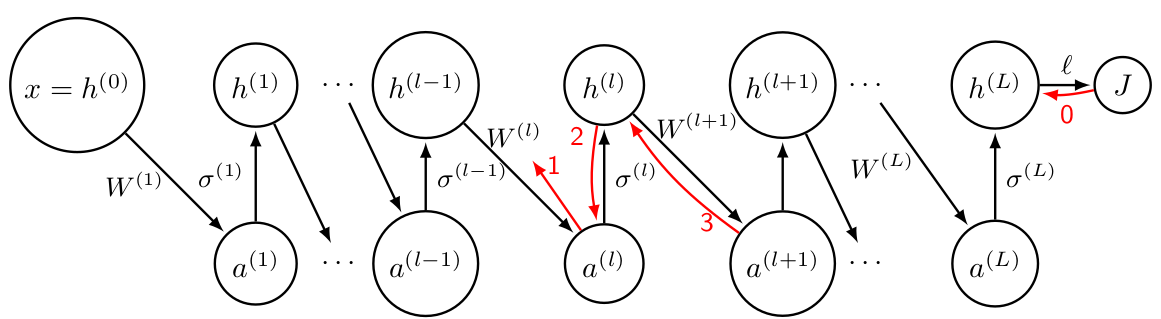
\includegraphics[width=\textwidth]{screenshot-backprop-figure}

For
each layer $l\in \{1, \dots, L\}$ we have:
\begin{eqnarray*}
  a^{(l)} &=&  W^{(l)} h^{(l-1)}, \\
  h^{(l)} &=& \sigma^{(l)}\left[ a^{(l)} \right].
\end{eqnarray*}
There are essentially four rules for computing gradients during
backpropagation (0-3).
  
\end{frame}

\begin{frame}
  \frametitle{Backprop rules}
  The rules 0--3 for backprop (from loss backwards):
\begin{description}
\item[Rule 0] computes $\nabla_{h^{(L)}} J$, which depends on the
  choice of the loss function $\ell$.
\item[Rule 1] computes
  $\nabla_{W^{(l)}} J$ using $\nabla_{a^{(l)}} J$, for any $l\in\{1,\dots,L\}$
\begin{eqnarray}
  \nabla_{w_k^{(l)}} J
  &=& \left(\nabla_{a^{(l)}} J\right)
      \left( h^{(l-1)} \right)^T \label{eq:grad-loss-w}
\end{eqnarray}
\item[Rule 2] computes
  $\nabla_{a^{(l)}} J$ using $\nabla_{h^{(l)}} J$, for any $l\in\{1,\dots,L\}$.
\begin{eqnarray}
  \nabla_{a^{(l)}} J
  &=& \left(\nabla_{h^{(l)}} J\right) \odot
      \label{eq:grad-loss-a}
      \left(\nabla_{a^{(l)}} h^{(l)} \right) 
  %&=& \left(\nabla_{h^{(l)}} J\right) \odot \left(h^{(l)}[1-h^{(l)}]\right).\label{eq:logistic-activation}
\end{eqnarray}
\item[Rule 3] computes
  $\nabla_{h^{(l)}} J$ using $\nabla_{a^{(l+1)}} J$, for any $l\in\{1,\dots,L-1\}$.
\begin{eqnarray}
  \nabla_{h^{(l)}} J
  &=& \left(\nabla_{a^{(l+1)}} J\right)
      \left(W^{(l+1)}\right)^T \label{eq:grad-loss-h}
\end{eqnarray}
\end{description}

\end{frame}

\end{document}